\documentclass[unicode,12pt,aspectratio=169]{beamer}

\usepackage{luatexja}% 日本語したい
\usepackage[haranoaji,no-math,deluxe,expert,nfssonly,match,scale=1.0]{luatexja-preset}
\renewcommand{\kanjifamilydefault}{\gtdefault}% 既定をゴシック体に

\usepackage{amssymb,amsmath,ascmac}

\usepackage{multirow}
\usepackage{lltjext}

\usepackage{siunitx}
\usepackage{physics}
\AtBeginDocument{\RenewCommandCopy\qty\SI}
\ExplSyntaxOn
\msg_redirect_name:nnn { siunitx } { physics-pkg } { none }
\ExplSyntaxOff

\usepackage{animate}
\usepackage{svg}
\usepackage{tikz}
\usepackage{xparse}
%%%%%%%%%%%%%%%%%%%%%%%
\graphicspath{{../fig/}}
%%%%%%%%%%%%%%%%%%%%%%%%%%%
\usetikzlibrary{shapes,arrows}
\usetikzlibrary{positioning}
\usetikzlibrary{angles,quotes}
\usetikzlibrary{math, calc}
\usetikzlibrary{decorations.markings,decorations.pathmorphing}
%% define fancy arrow. \tikzfancyarrow[<option>]{<text>}. ex: \tikzfancyarrow[fill=red!5]{hoge}
\tikzset{arrowstyle/.style n args={2}{inner ysep=0.1ex, inner xsep=0.5em, minimum height=2em, draw=#2, fill=black!20, font=\sffamily\bfseries, single arrow, single arrow head extend=0.4em, #1,}}
\NewDocumentCommand{\tikzfancyarrow}{O{fill=black!20} O{none}  m}{
\tikz[baseline=-0.5ex]\node [arrowstyle={#1}{#2}] {#3 \mathstrut};}

%目次スライド
% \AtBeginSection[]{
%   \frame{\tableofcontents[currentsection]}
% }
%アペンディックスのページ番号除去
\newcommand{\backupbegin}{
\newcounter{framenumberappendix}
\setcounter{framenumberappendix}{\value{framenumber}}
}
\newcommand{\backupend}{
\addtocounter{framenumberappendix}{-\value{framenumber}}
\addtocounter{framenumber}{\value{framenumberappendix}} 
}

%%%%%%%%%%%  theme  %%%%%%%%%%%
% \usetheme{Copenhagen}
\usetheme{metropolis}
% \usetheme{CambridgeUS}
% \usetheme{Berlin}

%%%%%%%%%%%  inner theme  %%%%%%%%%%%
% \useinnertheme{default}

% %%%%%%%%%%%  outer theme  %%%%%%%%%%%
\useoutertheme{default}
% \useoutertheme{infolines}

%%%%%%%%%%%  color theme  %%%%%%%%%%%
%\usecolortheme{structure}

%%%%%%%%%%%  font theme  %%%%%%%%%%%
\usefonttheme{professionalfonts}
%\usefonttheme{default}

%%%%%%%%%%%  degree of transparency  %%%%%%%%%%%
%\setbeamercovered{transparent=30}

%%%%%%%%%%%  numbering  %%%%%%%%%%%
% \setbeamertemplate{numbered}
\setbeamertemplate{navigation symbols}{}
\setbeamertemplate{footline}[frame number]

%%%%%%%%%%%%%%%%%%%%%%%%%%%%%%%%%%%
% \setbeamertemplate{items}[default]
\setbeamertemplate{enumerate item}[default]

% セクション名だけをTOCに出力
\setcounter{tocdepth}{1}



\title{第四章 線形動的粘弾性について}
\date{\empty}

\begin{document}

\section{複素表現の基礎}
\subsection{複素数と動的刺激}
\begin{frame}
	\frametitle{複素数の基礎（定義）}
	\footnotesize
	\begin{columns}[c, onlytextwidth]
		\column{.45\linewidth}
		\begin{block}{虚数$i$と複素数$z$の定義}
			\begin{itemize}
				\item 虚数とは：$i^2=-1$を満たす数
				\item 複素数とは：実数$x,y$ により\\以下のように表される数\\
				$z=x+iy$
				\item 複素平面上の一点として表される
			\end{itemize}
		\end{block}

		\column{.3\linewidth}
		\centering
			\scalebox{0.7}{\begin{tikzpicture}[scale=1.5]
				\coordinate (o) at (0,0) node at (o) [below left]{$o$};
				\coordinate (z) at (2,1) node at (z) [above]{$z=x+iy$};
				\coordinate (x) at (2,0) node at (x) [below]{$x$};
				\coordinate (y) at (0,1) node at (y) [left]{$y$};

				\fill (z) circle (1pt);

				\draw[->,>=stealth,semithick] (-1,0)--(2.5,0) node[right]{$\mathrm{Re}$}; %x軸
				\draw[->,>=stealth,semithick] (0,-1)--(0,2.5) node[above]{$\mathrm{Im}$}; %y軸
				
				\draw[dashed] (z)--(x);
				\draw[dashed] (z)--(y);
				\draw[red] (o)--(z);

				% \draw[thin] ([shift={(0,0)}]0:0.5) arc [radius=0.5, start angle = 0, end angle=30];
			\end{tikzpicture}}
		\column{.25\linewidth}
			% \begin{itembox}[l]{複素平面}
				\begin{itemize}
					\item 複素平面
					\item 横軸：実数軸
					\item 縦軸：虚数軸
				\end{itemize}
			% \end{itembox}
	\end{columns}

	\uncover<2>{
		\begin{itembox}[l]{\textbf{虚数を恐れずに、気楽に理解}}
		\begin{itemize}
			\item imaginary numberを「定義を満たす想像上の数」ととらえ、
			\item complex planeを「複合化した平面」と考える
		\end{itemize}
	\end{itembox}
	}
\end{frame}

\begin{frame}
	\frametitle{複素数の四則演算}

		2つの複素数に対して、四則演算は以下と定義される\\
		\uncover<2->{\alert{$i$を単なる記号として、虚数項と実数項を分けて計算しているだけ}}
		\vspace{-3mm}
		\begin{align*}
			z_1 = x_1+iy_1\\
			z_2 = x_2+iy_2
		\end{align*}
		\vspace{-8mm}
		\begin{itemize}
			\item<1-2> $z_1+z_2=(x_1+x_2) + i(y_1+y_2)$
			\item<1-2> $z_1-z_2=(x_1-x_2) + i(y_1-y_2)$
			\item<1,3> $z_1z_2=(x_1+iy_1)(x_2+iy_2)=x_1x_2-y_1y_2+i(x_1y_2+x_2y_1)$
			\item<1,4> $\dfrac{z_1}{z_2}=\dfrac{(x_1+iy_1)}{(x_2+iy_2)}=\dfrac{(x_1+iy_1)(x_2-iy_2)}{(x_2+iy_2)(x_2-iy_2)}$ \alert{分母を実数化し虚数項を分離}\\
			$=\dfrac{x_1x_2+y_1y_2}{x_2^2+y_2^2}+i\dfrac{-x_1y_2+x_2y_1}{x_2^2+y_2^2}$
		\end{itemize}
\end{frame}

\begin{frame}
	\frametitle{ガウス平面での和と差}
		\footnotesize
		\begin{columns}[c, onlytextwidth]
			\column{.48\linewidth}
			\begin{block}{2つの複素数の和と差は}
				\vspace{-3mm}
				\begin{align*}
					z_1 = x_1+iy_1\\
					z_2 = x_2+iy_2
				\end{align*}
				\vspace{-8mm}
				\begin{align*}
					z_1+z_2&=(x_1+x_2) + i(y_1+y_2)\\
					z_1-z_2&=(x_1-x_2) + i(y_1-y_2)
				\end{align*}
			\end{block}


			\uncover<2,3>{
				\begin{block}{ガウス平面での考え方}
					ベクトルと捉えることができ
					\begin{itemize}
						\item<2> 和はベクトルの和
						\item<3> 差はベクトルの差
					\end{itemize}
				\end{block}
				}
			\column{.48\linewidth}
			\centering
			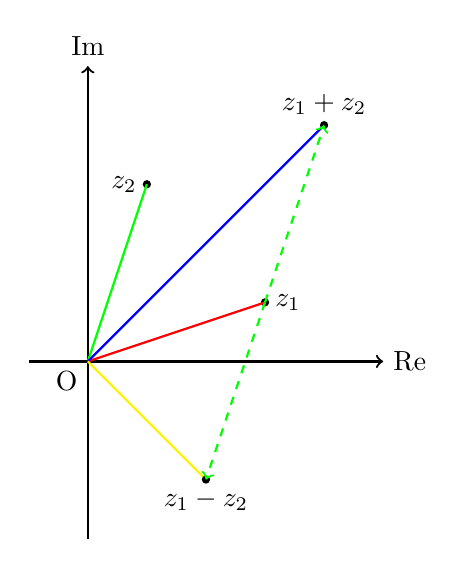
\begin{tikzpicture}[thick, scale=.75]
				% 軸
				\draw[->] (-1,0)--(5,0) node[right]{$\mathrm{Re}$}; %x軸
				\draw[->] (0,-3)--(0,5) node[above]{$\mathrm{Im}$}; %y軸
				\coordinate (o) at (0,0) node at (o) [below left]{$\mathrm{O}$};
				% z1
				\coordinate (z1) at (3,1) node at (z1) [right]{$z_1$};
				\fill[black] (z1) circle (2pt);
				\draw[red] (o)--(z1);
				% z2
				\coordinate (z2) at (1,3) node at (z2) [left]{$z_2$};
				\fill[black] (z2)circle (2pt);
				\draw[green] (o)--(z2);
				% z1+z2
				\coordinate<2> (z1p2) at ($(z1)+(z2)$) node at (z1p2) [above]{$z_1+z_2$};
				\draw<2>[blue] (o)--(z1p2);
				\fill<2>[black] (z1p2) circle (2pt);
				\draw<2>[->, dashed, green] (z1)--(z1p2);
				% z1-z2
				\coordinate<3> (z1m2) at ($(z1)-(z2)$) node at (z1m2) [below]{$z_1-z_2$};
				\draw<3>[yellow] (o)--(z1m2);
				\fill<3>[black] (z1m2) circle (2pt);
				\draw<3>[->, dashed, green] (z1)--(z1m2);
			\end{tikzpicture}
		\end{columns}
\end{frame}

\begin{frame}
	\frametitle{ガウス平面での極形式}
		\footnotesize
		\begin{columns}[c, onlytextwidth]
			\column{.48\linewidth}
			\begin{block}{平面座標系での極座標とは}
				\begin{itemize}
					\item 動径$r$と偏角$\theta$からなる座標
					\item 極形式とも呼ばれる
				\end{itemize}
			\end{block}

			\centering
			\scalebox{0.65}{\begin{tikzpicture}[thick, scale=1.2]
				% 軸
				\coordinate (o) at (0,0) node at (o) [below left]{$\mathrm{O}$};
				\coordinate (xm) at (4,0);
				\coordinate (ym) at (0,3);
				\draw[->] ($(o)+(-1,0)$)--(xm) node[right]{$x$}; %x軸
				\draw[->] ($(o)+(0,-1)$)--(ym) node[above]{$y$}; %y軸
				% z
				\coordinate (z) at (3,2) node at (z) [above]{$(r\cos(\theta), r\sin(\theta))$};
				\draw[red] (o)--(z) node at ($(o)!0.5!(z)$) [above]{$r$};
				\fill[black] (z) circle (2pt);
				% 補助線
				\draw[dashed] (z)--($(o)!(z)!(xm)$) node[below]{$r\cos(\theta)$};
				\draw[dashed] (z)--($(o)!(z)!(ym)$) node[left]{$r\sin(\theta)$};
				% 角度
				\draw pic[draw=black,angle eccentricity=1.5, angle radius=0.5cm, "\theta"]{angle=xm--o--z};
			\end{tikzpicture}}

			\vspace{-5mm}
			\begin{equation*}
				r=\sqrt{r^2\cos^2(\theta)+r^2\sin^2(\theta)}
			\end{equation*}
			\column<2>{.48\linewidth}
			\begin{block}{ガウス平面での極形式}
				\begin{itemize}
					\item 複素数$z=x+iy$の実部$x$と虚部$y$を
					\item それぞれ極座標表示し
					\item $z=r(\cos(\theta)+i\sin(\theta))$と表記
				\end{itemize}
			\end{block}

			\centering
			\scalebox{0.65}{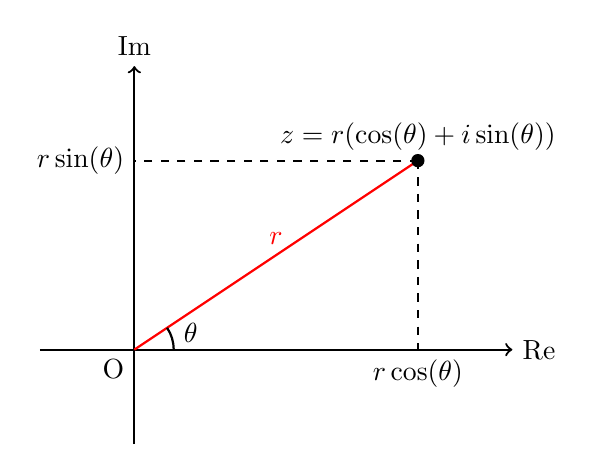
\begin{tikzpicture}[thick, scale=1.2]
				% 軸
				\coordinate (o) at (0,0) node at (o) [below left]{$\mathrm{O}$};
				\coordinate (xm) at (4,0);
				\coordinate (ym) at (0,3);
				\draw[->] ($(o)+(-1,0)$)--(xm) node[right]{$\mathrm{Re}$}; %x軸
				\draw[->] ($(o)+(0,-1)$)--(ym) node[above]{$\mathrm{Im}$}; %y軸
				% z
				\coordinate (z) at (3,2) node at (z) [above]{$z=r(\cos(\theta)+i\sin(\theta))$};
				\draw[red] (o)--(z) node at ($(o)!0.5!(z)$) [above]{$r$};
				\fill[black] (z) circle (2pt);
				% 補助線
				\draw[dashed] (z)--($(o)!(z)!(xm)$) node[below]{$r\cos(\theta)$};
				\draw[dashed] (z)--($(o)!(z)!(ym)$) node[left]{$r\sin(\theta)$};
				% 角度
				\draw pic[draw=black,angle eccentricity=1.5, angle radius=0.5cm, "$\theta$"]{angle=xm--o--z};
			\end{tikzpicture}}
		\end{columns}
\end{frame}

\begin{frame}
	\frametitle{ガウス平面の極形式での複素数の積}
		\footnotesize
			2つの複素数を極形式で表し
			\vspace{-3mm}
			\begin{align*}
				z_1=r_1\cos\theta_1+i r_1\sin\theta_1\\
				z_2=r_2\cos\theta_2+i r_2\sin\theta_2
			\end{align*}
			% \vspace{-3mm}
			その積を求める
			\vspace{-3mm}
			\begin{align*}
				z_1z_2&=\left(r_1\cos\theta_1+i r_1\sin\theta_1\right)\left(r_2\cos\theta_2+i r_2\sin\theta_2\right)\\
				&=r_1r_2\cos\theta_1\cos\theta_2-r_1r_2\sin\theta_1\sin\theta_2\\
				&\quad\quad+i\left(r_1r_2\sin\theta_1\cos\theta_2+r_1r_2\cos\theta_1\sin\theta_2\right)
			\end{align*}
			ここで、以下の加法定理を用いて、
			\vspace{-3mm}
			\begin{align*}
				\sin(\alpha+\beta)=\sin\alpha\cos\beta+\cos\alpha\sin\beta\\
				\cos(\alpha+\beta)=\cos\alpha\cos\beta-\sin\alpha\sin\beta
			\end{align*}
			結局、
			\vspace{-3mm}
			\begin{align*}
				z_1z_2&=r_1r_2 \left(\cos(\theta_1+\theta_2)+i\sin(\theta_1+\theta_2)\right)
			\end{align*}
\end{frame}

\begin{frame}
	\frametitle{ガウス平面の極形式での複素数の積}
		\footnotesize
		\begin{columns}[c, onlytextwidth]
			\column{.58\linewidth}
			2つの複素数を極形式で表し
			% \vspace{-3mm}
			\begin{align*}
				z_1=r_1\cos(\theta_1)+i r_2\sin(\theta_1)\\
				z_2=r_2\cos(\theta_2)+i r_2\sin(\theta_2)
			\end{align*}

			その積を求める
			% \vspace{-3mm}
			\begin{align*}
				z_1z_2&=r_1r_2 (\cos(\theta_1+\theta_2)+i\sin(\theta_1+\theta_2))
			\end{align*}
			
			\begin{block}<2>{この解は以下の複素数}
				\begin{itemize}
					\item 動径（絶対値）が各動径の積$r_1r_2$
					\item 偏角が各偏角の和$\theta_1+\theta_2$
				\end{itemize}
			\end{block}
			
			\column{.4\linewidth}
			\centering
			\scalebox{0.8}{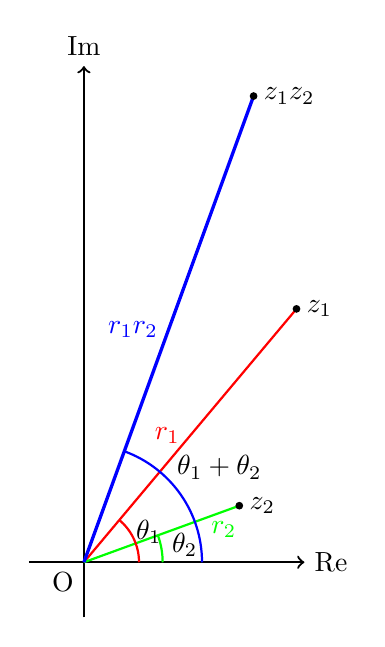
\begin{tikzpicture}[thick, scale=1.4]
				% 軸
				\coordinate (o) at (0,0) node at (o) [below left]{$\mathrm{O}$};
				\coordinate (xm) at (2,0);
				\coordinate (ym) at (0,4.5);
				\draw[->] ($(o)+(-.5,0)$)--(xm) node[right]{$\mathrm{Re}$}; %x軸
				\draw[->] ($(o)+(0,-.5)$)--(ym) node[above]{$\mathrm{Im}$}; %y軸
				% z1
				\coordinate (z1) at (50:3) node at (z1) [right]{$z_1$};
				\draw[red] (o)--(z1) node at ($(o)!0.5!(z1)$) [left]{$r_1$};
				\fill[black] (z1) circle (1pt);
				% z2
				\coordinate (z2) at (20:1.5) node at (z2) [right]{$z_2$};
				\draw[green] (o)--(z2) node at ($(o)!0.9!(z2)$) [below]{$r_2$};
				\fill[black] (z2) circle (1pt);
				% z1z2
				\coordinate<2> (z1z2) at (70:4.5) node at (z1z2) [right]{$z_1z_2$};
				\draw<2>[very thick, blue] (o)--(z1z2) node at ($(o)!0.5!(z1z2)$) [left]{$r_1r_2$};
				\fill<2>[black] (z1z2) circle (1pt);
				% % 補助線
				% \draw[dashed] (z)--($(o)!(z)!(xm)$) node[below]{$r\cos(\theta)$};
				% \draw[dashed] (z)--($(o)!(z)!(ym)$) node[left]{$r\sin(\theta)$};
				% 角度
				\draw pic[draw=red,angle eccentricity=1.3, angle radius=0.7cm, "$\theta_1$"]{angle=xm--o--z1};
				\draw pic[draw=green,angle eccentricity=1.3, angle radius=1.cm, "$\theta_2$"]{angle=xm--o--z2};
				\draw<2> pic[draw=blue,angle eccentricity=1.4, angle radius=1.5cm, "$\theta_1+\theta_2$"]{angle=xm--o--z1z2};
			\end{tikzpicture}}
		\end{columns}
\end{frame}

\begin{frame}
	\frametitle{ガウス平面の極形式での複素数の商}
		\footnotesize
			% 2つの複素数を極形式で表し
			% \vspace{-3mm}
			% \begin{align*}
			% 	z_1=r_1\cos\theta_1+i r_1\sin\theta_1\\
			% 	z_2=r_2\cos\theta_2+i r_2\sin\theta_2
			% \end{align*}
			% \vspace{-3mm}
			極形式で複素数の商を求める
			% \vspace{-3mm}
			\begin{align*}
				\dfrac{z_1}{z_2}&=\dfrac{r_1\cos\theta_1+i r_1\sin\theta_1}{r_2\cos\theta_2+i r_2\sin\theta_2}\\
				&=\dfrac{r_1(\cos\theta_1+i\sin\theta_1)(\cos\theta_2-i\sin\theta_2)}{r_2(\cos\theta_2+i\sin\theta_2)(\cos\theta_2-i\sin\theta_2)}\\
				&=\dfrac{r_1[(\cos\theta_1\cos\theta_2 +\sin\theta_1 \sin\theta_2)+i(\sin\theta_1\cos\theta_2-\cos\theta_1 \sin\theta_2)]}{r_2(\cos^2\theta_2+\sin^2\theta_2)}
			\end{align*}
			$\cos^2\theta_2+\sin^2\theta_2=1$および以下の加法定理を用いることで、
			% \vspace{-3mm}
			\begin{align*}
				\sin(\alpha-\beta)=\sin\alpha\cos\beta-\cos\alpha\sin\beta\\
				\cos(\alpha-\beta)=\cos\alpha\cos\beta+\sin\alpha\sin\beta
			\end{align*}
			結局、
			% \vspace{-3mm}
			\begin{align*}
				\dfrac{z_1}{z_2}=\dfrac{r_1}{r_2} \left(\cos(\theta_1-\theta_2)+i\sin(\theta_1-\theta_2)\right)
			\end{align*}
\end{frame}

\begin{frame}
	\frametitle{ガウス平面の極形式での複素数の商}
		\footnotesize
		\begin{columns}[c, onlytextwidth]
			\column{.58\linewidth}
			2つの複素数を極形式で表し
			% \vspace{-3mm}
			\begin{align*}
				z_1=r_1\cos(\theta_1)+i r_2\sin(\theta_1)\\
				z_2=r_2\cos(\theta_2)+i r_2\sin(\theta_2)
			\end{align*}

			その商を求める
			% \vspace{-3mm}
			\begin{align*}
				\dfrac{z_1}{z_2}=\dfrac{r_1}{r_2} (\cos(\theta_1-\theta_2)+i\sin(\theta_1-\theta_2))
			\end{align*}
			
			\begin{block}<2>{この解は以下の複素数}
				\begin{itemize}
					\item 動径が各動径の商$\dfrac{r_1}{r_2}$
					\item 偏角が各偏角の差$\theta_1-\theta_2$
				\end{itemize}
			\end{block}
			\column{.4\linewidth}
			\centering
			\scalebox{0.8}{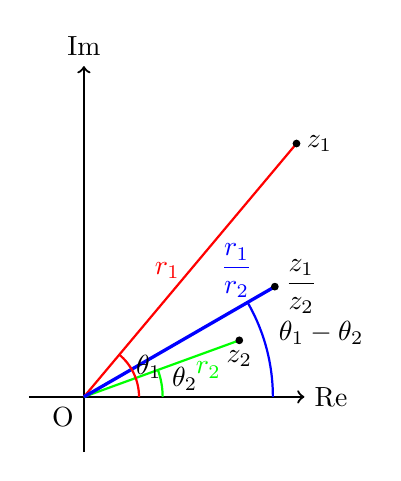
\begin{tikzpicture}[thick, scale=1.4]
				% 軸
				\coordinate (o) at (0,0) node at (o) [below left]{$\mathrm{O}$};
				\coordinate (xm) at (2,0);
				\coordinate (ym) at (0,3);
				\draw[->] ($(o)+(-.5,0)$)--(xm) node[right]{$\mathrm{Re}$}; %x軸
				\draw[->] ($(o)+(0,-.5)$)--(ym) node[above]{$\mathrm{Im}$}; %y軸
				% z1
				\coordinate (z1) at (50:3) node at (z1) [right]{$z_1$};
				\draw[red] (o)--(z1) node at ($(o)!0.5!(z1)$) [left]{$r_1$};
				\fill[black] (z1) circle (1pt);
				% z2
				\coordinate (z2) at (20:1.5) node at (z2) [below]{$z_2$};
				\draw[green] (o)--(z2) node at ($(o)!0.8!(z2)$) [below]{$r_2$};
				\fill[black] (z2) circle (1pt);
				% z1z2
				\coordinate<2> (z1z2) at (30:2) node at (z1z2) [right]{$\dfrac{z_1}{z_2}$};
				\draw<2>[very thick, blue] (o)--(z1z2) node at ($(o)!0.8!(z1z2)$) [above]{$\dfrac{r_1}{r_2}$};
				\fill<2>[black] (z1z2) circle (1pt);
				% 角度
				\draw pic[draw=red,angle eccentricity=1.3, angle radius=0.7cm, "$\theta_1$"]{angle=xm--o--z1};
				\draw pic[draw=green,angle eccentricity=1.3, angle radius=1.cm, "$\theta_2$"]{angle=xm--o--z2};
				\draw<2> pic[draw=blue,angle eccentricity=1.3, angle radius=2.4cm, "$\theta_1-\theta_2$"]{angle=xm--o--z1z2};
			\end{tikzpicture}}
		\end{columns}
\end{frame}

\begin{frame}
	\frametitle{ガウス平面上の単位円とオイラーの公式}
		\footnotesize
		\begin{columns}[c, onlytextwidth]
			\column{.48\linewidth}
			オイラーの公式の右辺は、ガウス平面での動径$r=1$の極表示と同型
			\vspace{-2mm}
			\begin{align*}
				\exp(i\theta)=cos\theta+i\sin\theta
			\end{align*}
			% \vspace{-2mm}
			\uncover<2->{$\theta$を変数と見ればガウス平面上の単位円

			\centering
			\scalebox{0.6}{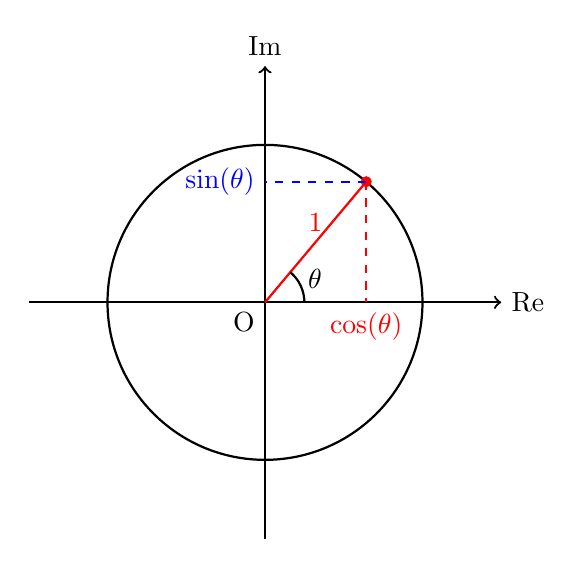
\begin{tikzpicture}[thick, scale=2]
				% 軸
				\coordinate (o) at (0,0) node at (o) [below left]{$\mathrm{O}$};
				\coordinate (xm) at (1.5,0);
				\coordinate (ym) at (0,1.5);
				\draw[->] ($-1*(xm)$)--(xm) node[right]{$\mathrm{Re}$}; %x軸
				\draw[->] ($-1*(ym)$)--(ym) node[above]{$\mathrm{Im}$}; %y軸
				% 円
				\draw (o) circle [radius=1];
				% z1
				\coordinate (z) at (50:1);
				\draw[red] (o)--(z) node at ($(o)!0.5!(z)$) [above]{$1$};
				\fill[red] (z) circle (1pt);
				% 補助線
				\draw[dashed, red] (z)--($(o)!(z)!(xm)$) node[below]{$\cos(\theta)$};
				\draw[dashed, blue] (z)--($(o)!(z)!(ym)$) node[left]{$\sin(\theta)$};
				% 角度
				\draw pic[draw=black, angle eccentricity=1.4, angle radius=.5cm, "$\theta$"]{angle=xm--o--z};
			\end{tikzpicture}}}
			\column{.48\linewidth}
				\only<3>{
					\begin{itemize}
						\item 以下の類似性を利用して、
						\begin{itemize}
							\footnotesize
							\item 指数関数の乗除算が指数の加減に対応すること
							\item 極表示での複素数の乗除算が迎角の加減となること
						\end{itemize}
						\item 円運動を$\exp(i\theta)$で記述すると数式展開に有用なことが知られている。
						\begin{itemize}
							\footnotesize
							\item 当然、波を記述可能。
							\item 位相差も自然に表現できる。
						\end{itemize}
					\end{itemize}
				}
				% \only<4->{
				% 	以下の2つの複素数を考える。
				% 	\vspace{-3mm}
				% 	\begin{align*}
				% 		\exp(i\theta_1)=\cos\theta_1+i\sin\theta_1\\
				% 		\exp(i\theta_2)=\cos\theta_2+i\sin\theta_2
				% 	\end{align*}
				% }
				% \only<4>{	
				% 		\begin{equation*}
				% 			\exp(i\theta_1)\exp(i\theta_2)=\exp(i\theta_1+i\theta2)
				% 		\end{equation*}
				% }
				% \only<5>{	
				% 		\begin{equation*}
				% 			\dfrac{\exp(i\theta_1)}{\exp(i\theta_2)}=\exp(i\theta_1-i\theta2)
				% 		\end{equation*}
				% }
				% \only<4->{
				% \centering
				% \scalebox{0.6}{\begin{tikzpicture}[thick, scale=2]
				% 	% 軸
				% 	\coordinate (o) at (0,0) node at (o) [below left]{$\mathrm{O}$};
				% 	\coordinate (xm) at (1.5,0);
				% 	\coordinate (ym) at (0,1.5);
				% 	\draw[->] ($-1*(xm)$)--(xm) node[right]{$\mathrm{Re}$}; %x軸
				% 	\draw[->] ($-1*(ym)$)--(ym) node[above]{$\mathrm{Im}$}; %y軸
				% 	% 円
				% 	\draw (o) circle [radius=1];
				% 	% z1
				% 	\coordinate (z1) at (45:1) node at (z1) [above right]{$e^{i\theta_1}$};
				% 	\draw[red] (o)--(z1);
				% 	\fill[red] (z1) circle (1pt);
				% 	% z2
				% 	\coordinate (z2) at (70:1) node at (z2) [above right]{$e^{i\theta_2}$};
				% 	\draw[green] (o)--(z2);
				% 	\fill[green] (z2) circle (1pt);
				% 	% z1m2
				% 	\coordinate<4> (z1m2) at (115:1) node at (z1m2) [above]{$e^{(i\theta_1+i\theta_2)}$};
				% 	\draw<4>[blue] (o)--(z1m2);
				% 	\fill<4>[blue] (z1m2) circle (1pt);
				% 	% z1d2
				% 	\coordinate<5> (z1d2) at (-25:1) node at (z1d2) [right]{$\dfrac{e^{i\theta_1}}{e^{i\theta_2}}$};
				% 	\draw<5>[blue] (o)--(z1d2);
				% 	\fill<5>[red] (z1d2) circle (1pt);
				% 	% 角度
				% 	\draw pic[draw=black, angle eccentricity=1.5, angle radius=.3cm, "$\theta_1$"]{angle=xm--o--z1};
				% 	\draw pic[draw=green, angle eccentricity=1.4, angle radius=.7cm, "$\theta_2$"]{angle=xm--o--z2};
				% 	\draw<4> pic[draw=blue, angle eccentricity=1.3, angle radius=1.2cm, "$\theta_1+\theta_2$"]{angle=xm--o--z1m2};
				% 	\draw<5> pic[draw=blue, angle eccentricity=1.7, angle radius=.8cm, "$\theta_1-\theta_2$"]{angle=z1d2--o--xm};
				% \end{tikzpicture}}}
		\end{columns}
\end{frame}

% \begin{frame}
% 	\frametitle{ガウス平面上の単位円とオイラーの公式}
% 		\footnotesize
% 		\begin{columns}[c, onlytextwidth]
% 			\column{.48\linewidth}
% 			オイラーの公式の右辺は、ガウス平面での動径$r=1$の極表示と同型
% 			\vspace{-2mm}
% 			\begin{align*}
% 				\exp(i\theta)=cos\theta+i\sin\theta
% 			\end{align*}
% 			% \vspace{-2mm}
% 			\uncover<2->{$\theta$を変数と見ればガウス平面上の単位円

% 			\centering
% 			\scalebox{0.6}{\begin{tikzpicture}[thick, scale=2]
% 				% 軸
% 				\coordinate (o) at (0,0) node at (o) [below left]{$\mathrm{O}$};
% 				\coordinate (xm) at (1.5,0);
% 				\coordinate (ym) at (0,1.5);
% 				\draw[->] ($-1*(xm)$)--(xm) node[right]{$\mathrm{Re}$}; %x軸
% 				\draw[->] ($-1*(ym)$)--(ym) node[above]{$\mathrm{Im}$}; %y軸
% 				% 円
% 				\draw (o) circle [radius=1];
% 				% z1
% 				\coordinate (z) at (50:1);
% 				\draw[red] (o)--(z) node at ($(o)!0.5!(z)$) [above]{$1$};
% 				\fill[red] (z) circle (1pt);
% 				% 補助線
% 				\draw[dashed, red] (z)--($(o)!(z)!(xm)$) node[below]{$\cos(\theta)$};
% 				\draw[dashed, blue] (z)--($(o)!(z)!(ym)$) node[left]{$\sin(\theta)$};
% 				% 角度
% 				\draw pic[draw=black, angle eccentricity=1.4, angle radius=.5cm, "$\theta$"]{angle=xm--o--z};
% 			\end{tikzpicture}}}
% 			\column{.48\linewidth}
% 				\only<3>{
% 					\begin{itemize}
% 						\item 以下の類似性を利用して、
% 						\begin{itemize}
% 							\footnotesize
% 							\item 指数関数の乗除算が指数の加減に対応すること
% 							\item 極表示での複素数の乗除算が迎角の加減となること
% 						\end{itemize}
% 						\item 円運動を$\exp(i\theta)$で記述すると数式展開に有用なことが知られている。
% 						\begin{itemize}
% 							\footnotesize
% 							\item 当然、波を記述可能。
% 							\item 位相差も自然に表現できる。
% 						\end{itemize}
% 					\end{itemize}
% 				}
% 				\only<4->{
% 					以下の2つの複素数を考える。
% 					\vspace{-3mm}
% 					\begin{align*}
% 						\exp(i\theta_1)=\cos\theta_1+i\sin\theta_1\\
% 						\exp(i\theta_2)=\cos\theta_2+i\sin\theta_2
% 					\end{align*}
% 				}
% 				\only<4>{	
% 						\begin{equation*}
% 							\exp(i\theta_1)\exp(i\theta_2)=\exp(i\theta_1+i\theta2)
% 						\end{equation*}
% 				}
% 				\only<5>{	
% 						\begin{equation*}
% 							\dfrac{\exp(i\theta_1)}{\exp(i\theta_2)}=\exp(i\theta_1-i\theta2)
% 						\end{equation*}
% 				}
% 				\only<4->{
% 				\centering
% 				\scalebox{0.6}{\begin{tikzpicture}[thick, scale=2]
% 					% 軸
% 					\coordinate (o) at (0,0) node at (o) [below left]{$\mathrm{O}$};
% 					\coordinate (xm) at (1.5,0);
% 					\coordinate (ym) at (0,1.5);
% 					\draw[->] ($-1*(xm)$)--(xm) node[right]{$\mathrm{Re}$}; %x軸
% 					\draw[->] ($-1*(ym)$)--(ym) node[above]{$\mathrm{Im}$}; %y軸
% 					% 円
% 					\draw (o) circle [radius=1];
% 					% z1
% 					\coordinate (z1) at (45:1) node at (z1) [above right]{$e^{i\theta_1}$};
% 					\draw[red] (o)--(z1);
% 					\fill[red] (z1) circle (1pt);
% 					% z2
% 					\coordinate (z2) at (70:1) node at (z2) [above right]{$e^{i\theta_2}$};
% 					\draw[green] (o)--(z2);
% 					\fill[green] (z2) circle (1pt);
% 					% z1m2
% 					\coordinate<4> (z1m2) at (115:1) node at (z1m2) [above]{$e^{(i\theta_1+i\theta_2)}$};
% 					\draw<4>[blue] (o)--(z1m2);
% 					\fill<4>[blue] (z1m2) circle (1pt);
% 					% z1d2
% 					\coordinate<5> (z1d2) at (-25:1) node at (z1d2) [right]{$\dfrac{e^{i\theta_1}}{e^{i\theta_2}}$};
% 					\draw<5>[blue] (o)--(z1d2);
% 					\fill<5>[red] (z1d2) circle (1pt);
% 					% 角度
% 					\draw pic[draw=black, angle eccentricity=1.5, angle radius=.3cm, "$\theta_1$"]{angle=xm--o--z1};
% 					\draw pic[draw=green, angle eccentricity=1.4, angle radius=.7cm, "$\theta_2$"]{angle=xm--o--z2};
% 					\draw<4> pic[draw=blue, angle eccentricity=1.3, angle radius=1.2cm, "$\theta_1+\theta_2$"]{angle=xm--o--z1m2};
% 					\draw<5> pic[draw=blue, angle eccentricity=1.7, angle radius=.8cm, "$\theta_1-\theta_2$"]{angle=z1d2--o--xm};
% 				\end{tikzpicture}}}
% 		\end{columns}
% \end{frame}

\begin{frame}
	\frametitle{$\exp(i\theta)$による円運動}
		\small
		\begin{itemize}
			\item 「複素平面上で原点から単位円上の一点へ伸びたベクトル」
			\item $\textcolor{red}{\theta}$を変数として単位円上をグルグル回転
		\end{itemize}
		
		\centering
		\only<1>{
			\scalebox{0.7}{
				\begin{tikzpicture}[thick, scale=2]
					% 軸
					\coordinate (o) at (0,0) node at (o) [below left]{$\mathrm{O}$};
					\coordinate (xm) at (1.5,0);
					\coordinate (ym) at (0,1.5);
					\draw[->] ($-1*(xm)$)--(xm) node[right]{$\mathrm{Re}$}; %x軸
					\draw[->] ($-1*(ym)$)--(ym) node[above]{$\mathrm{Im}$}; %y軸
					% 円
					\draw (o) circle [radius=1];
					% z1
					\coordinate (z1) at (45:1);
					\draw[->] (o)--(z1);
					% \fill[red] (z1) circle (1pt);
					%円弧
					\draw[blue, very thick, <->] (20:1.2) arc (20:70:1.2);
					% 角度
					\draw pic[draw=red, angle eccentricity=1.4, angle radius=.5cm, "$\textcolor{red}{\theta}$"]{angle=xm--o--z1};
					% 
					\draw (2.7,0) node[font=\LARGE]{$=\exp(i\textcolor{red}{\theta})$};
				\end{tikzpicture}
			}
			}
		\only<2>{
			\animategraphics[loop, width=0.6\textwidth, autoplay]{20}{circle_sine/image_}{001}{060}
			}
\end{frame}

\begin{frame}
	\frametitle{「複素数とガウス平面」にかんするまとめ}

	\begin{boxnote}
		\begin{itemize}
			\item ポイント
			\begin{itemize}
				\item $i$を単に想像上の数と考えてお気楽に扱う
				\item 実数と虚数の二項になるように式変形
			\end{itemize}
			\item ガウス平面での極表現
			\begin{itemize}
				\item 積が偏角の和
				\item 商が偏角の差
			\end{itemize}
			\item オイラーの公式を用いた単位円
			\begin{itemize}
				\item $\exp(i\theta)$で自然に波動を表現
			\end{itemize}
		\end{itemize}		
	\end{boxnote}
\end{frame}

\end{document}